\section{Theorie}
\label{sec:Theorie}
    Die Funktionsweise des Diodenlasers basiert auf theoretischen Grundlagen aus der Quantenmechanik, sowie Atom- und Festkörperphysik.
    %Die für die technische Realisierbarkeit des Diodenlasers nötige Halbleitertechnik gilt als Schlüsseltechnologie der ersten Quantenrevolution.\\
    Im folgenden Abschnitt werden diese Grundlagen vorgestellt und zum Verständnis der Funktionsweise des Diodenlasers erläutert.
    


    % \subsection{Kohärenz}
    %     Licht ist kohärent, wenn die Photonen des Lichts in allen Quantenzahlen übereinstimmen. \textbf{QUELLE}%reicht das nicht lol?

        %Die Quantenmechanik liefert die Erkenntnis, dass das Photon, welches bei der stimulierten Emission frei wird, die gleiche Phasenbeziehung, Ausbreitungsrichtung und Frequenz hat wie das einfallende, induzierende Photon.
        %Tatsächlich stimmen die beiden Photonen in jeder Quantenzahl überein. Diese Identität der Quantenzahlen und des Verhaltens der Photonen wird als \textbf{Kohärenz} bezeichnet.\\
        %Kohärenz ist allerdings eine Eigenschaft, die durch externe Einflüsse behindert, eingeschränkt oder aufgehoben werden kann. Brechung und Beugung von Licht, Streuung an den Luftmolekülen sowie Interferenz mit externer Strahlung können Änderungen der Quantenzahlen verursachen.
        %Bereits minimale Abweichungen der Phase oder Frequenz, entwickeln sich mit fortschreitender Zeit weiter auseinander und sorgen für immer geringere Kohärenz. 
        %\\
        %Die Stabilität der Phase und Frequenz eines Lasers fällt unter die \textbf{zeitliche Kohärenz}. Aus ihr ergibt sich die Linienbreite und die Kohärenzlänge.
        %Die Kohärenzlänge ist die Entfernung, die sich aus der Lichtgeschwindigkeit $c$ und der Linienbreite $\symup{\Delta}\nu$ berechnet in der Form
        %\begin{equation}
        %    l = c\cdot\symup{\Delta}t = \frac{c}{\symup{\Delta}\nu}\,\mathrm{.}
        %\end{equation}
        %Davon abgesehen spielt auch die Frage eine Rolle, wie gut das Licht seine uhrsprüngliche Fokussierung beibehält. Dies wird als \textbf{räumliche Kohärenz} bezeichnet.
        %\\
        %Laserlicht weist sowohl sehr hohe räumliche als auch zeitliche Kohärenz auf. Erstere ist technisch begrenzt durch den optischen Strahlengang des Laserstrahls, vor allem der Laserblende.
        %Die zeitliche Kohärenz kann über die Kohärenzlänge quantifiziert werden. Bei Lassern liegt sie im Bereich von $\qty{300000}{\kilo\meter}$ \cite[325]{haken_wolf_2004}.
    \subsection{Absorption und Emission elektromagnetischer Stahlung}
        % Im Jahr 1900 formulierte Max Planck sein Strahlungsgesetz für das elektromagnetische Spektrum eines Schwarzkörperstahlers.
        % Dabei traf er die Annahme, dass die Wechselwirkung zwischen Licht und Materie durch diskrete Energien der Form $E = \symup{h}\cdot\nu$ beschrieben werden kann \cite[52]{haken_wolf_2004}.
        % Dabei ist $\nu$ die Frequenz des Lichts und $\symup{h}$ das Planck'sche Wirkungsquantum.
        % \\
        % Auf diese Interpretation stützt sich auch das Bohr'sche Atommodell (1913), welches in drei Postulaten den Elektronen diskrete Energieniveaus vorgibt.
        % Dies liefert eine Erklärung für die diskreten Emissionsspektren, die für jedes chemische Element verschieden und einzigartig sind.
        % Die Übergangsenergie, die nötig ist, um ein Elektron vom Energieniveau $E_1$ in das höhere Energieniveau $E_2$ anzuheben beträgt
        % \begin{equation}
        %     \symup{\Delta}E = E_2 - E_1 = h\nu\,\mathrm{.}
        %     \label{eqn:planck}
        % \end{equation}
        % Um den Übergang von $E_1$ nach $E_2$ zu realisieren, muss also dem Elektron in $E_1$ die Energie $\symup{\Delta}E$ zugeführt werden.
        % Der umgekehrte Prozess setzt entsprechend Energie $\symup{\Delta}E$ frei \cite[95]{haken_wolf_2004}.
        % \\
        % Anhand des Photoeffekts konnte Albert Einstein die Lichtquantenhypothese aufstellen und zeigen, dass elektromagnetische Strahlung nicht nur durch Wellen, sondern auch durch Lichtteilchen mit diskreten, frequenzabhängigen Energien beschrieben werden kann.
        % Für die im Diodenlaser auftretenden Prozesse ist diese Betrachtungsweise besonders relevant, da sie ermöglicht, die Wechselwirkung zwischen Licht und Materie als Prozess mit Photonenaustausch zu beschreiben.
        % \\
        %Alle bekannten chemischen Elemente besitzen auf atomarer Ebene diskrete Energieniveaus, welche abhängig sind von ihrer Elektronenkonfiguration.
        %In vielen Experimenten konnte nachgewiesen werden, dass diese Niveaus auf vielfältige Weise angeregt und manipuliert werden können.
        %Durch Bestrahlung der Atome mit Photonen kann beeinflusst werden, welche Energieniveaus die Elektronen der Atomhülle besetzen.
        Elektronen in Atomhüllen befinden sich auf diskreten Energieniveaus. 
        Sie können durch Absorbtion sowie stimulierte und sponane Emission zwischen zwei Energieniveaus wechseln. 
        Dabei wird entweder ein Photon absorbiert oder emittiert.
        In \autoref{fig:atomanregungen} werden die drei Prozesse anhand eines Zwei-Niveau-Systems veranschaulicht.
         Die stimulierte Emission wird dort \enquote{induzierte} Emission genannt.
        Die Energiedifferenz des Übergangs zwischen den Energieniveaus $E_1$ und $E_2$ ist durch
        \begin{equation}
            \symup{\Delta}E = E_2 - E_1 = h f
            \label{eqn:planck}
        \end{equation}
        gegeben.
        Dabei ist $\symup{h}$ das Planck'sche Wirkungsquantum und $f$ die Frequenz des Photons, dessen Energie der Energiedifferenz des Übergangs entspricht~\cite[59]{haken_wolf_2004}.
        \\
        %Bei den Prozessen, die mittels Photonenaustausch das Energieniveau eines Elektrons in der Atomhülle ändern können, wird unterschieden zwischen der Absorption, der spontanen Emission und der stimulierten Emission \cite[53]{haken_wolf_2004}.
        %In \autoref{fig:atomanregungen} werden die drei Prozesse anhand eines Zwei-Niveau-Systems veranschaulicht. Die stimulierte Emission wird dort \enquote{induzierte} Emission genannt. Diese Formulierung ist ebenfalls üblich und beschreibt den gleichen Prozess.
        %Für die Funktionsweise eines Lasers sind allerdings Drei- oder Vier-Niveau-Systeme nötig. Diese werden in  Unterabschnitt \ref{sec:systeme} behandelt. 
        \begin{figure}
            \centering
            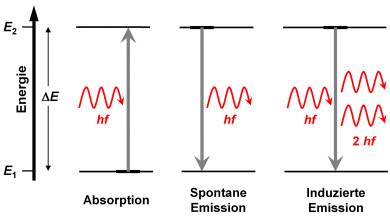
\includegraphics[width=0.5\textwidth]{content/images/atomanregungen.png}
            \caption{Absorption, spontane Emission und stimulierte Emission in einem Zwei-Niveau-System~\cite{seos_project}.}
            \label{fig:atomanregungen}
        \end{figure}
        \FloatBarrier\noindent
        Bei der \textbf{Absorption} trifft ein Photon mit der Energiedifferenz $\increment E$ der beiden Energieniveaus auf das Atom und regt so das Elektron von Energienivau $E_1$ in $E_2$ an~\cite[59]{haken_wolf_2004}.
         %handelt es sich um den durch \autoref{eqn:planck} von rechts nach links beschriebenen Prozess.
       % Ein auf die Materie treffendes Photon der Energie $\symup{h}\nu$ wechselwirkt mit dem Elektron $\Psi_1$, das sich im Energieniveau $E_1$ befindet.
        %Wenn es ein höheres Energieniveau $E_2$ gibt, dessen energetischer Abstand $\symup{\Delta}E$ von $E_1$ gleich der Energie des einfallenden Photons ist, dann ändert sich der Zustand des Elektrons.
        %Es befindet sich nun im Zustand $\Psi_2$.
        %Dieser Übergang findet nur mit einer gewissen Wahrscheinlichkeit statt, die sich mittels der zeitabhängigen Störungstheorie und Fermi's \enquote{Goldener Regel} ermitteln lässt. 
        %Dabei ist die Zunahme der Absorptionsrate linear proportional zur Anzahl der einfallenden Photonen \cite[293]{schwabl_1992}.\\
        %Viele der 
        \\
        %Energieniveaus, die durch Absorption angeregt werden können, sind instabil. 
        %Die angeregten Elektronen befinden sich in einem energetisch nicht optimalen Zustand. 
        Elektronen verlassen den angeregent Zustand nach einer mittleren Lebensauer wieder, ohne äußere Einflüsse.
        Dabei wird ein Photon der Energie $\increment E$ emittiert und das Elektron fällt wieder in das niedrigere Energieniveau $E_1$.
        Dieser Prozess wird \textbf{spontane Emission} genannt~\cite[60]{haken_wolf_2004}.
        \\
        %Dabei sendet ein System, welches sich im höheren Energieniveau $\Psi_2$ befindet ein Photon mit der Energie $\symup{\Delta}E = \symup{h}\nu $ aus und fällt dabei in den niedrigeren Zustand $\Psi_1$ \cite[149]{yariv_1991}. 
        %Die Richtung, in die das Photon emittiert wird, ist zufällig und wird als Fluoreszenzlicht wahrgenommen.
        %Die Wahrscheinlichkeit, mit der dies geschiet, lässt sich ebenfalls störungstheoretisch berechnen.
        %Dabei kann jedem Übergang, der durch spontane Emission stattfindet, eine mittlere Lebensdauer $\tau$ zugeordnet werden.
        %Diese Lebensdauer ist abhängig von der Energiedifferenz des betrachteten Übergangs. Es folgt der Zusammenhang
        %\begin{equation}
        %    \symup{\Delta}E \propto \frac{\symup{h}}{\tau}\,\mathrm{.}
        %\end{equation}
        %Je höher also die Energiedifferenz zwischen angeregtem Zustand und Grundzustand, desto kürzer ist die Lebensdauer des Zustands, bevor er durch spontane Emission zerfällt \cite[95]{schwabl_1992}.\\
        Die \textbf{stimulierte Emission} findet statt, wenn ein Photon mit der Energie $\symup{\Delta}E$ auf das System trifft, welches sich bereits im angeregten Energieniveau $E_2$ befindet. 
        Durch das einfallende Photon stimuliert, fällt auch hier das System in das niedrigere Energieniveau $E_1$ unter Emission eines weiteren Photons der Energie $\increment E$.
        Die Photonenzahl und Intensität verdoppeln sich.
        Alle Quantenzahlen des emittierten Photons sind gleich denen des einfallenden Photons.
        Das entstehende Licht ist kohärent.~\cite[31]{eichler_2015}.
        
        %im Zustand $\Psi_2$ trifft. 
        %Dieses Photon wird nicht absorbiert, sondern löst den Übergang des Systems in den Zustand $\Psi_1$ aus, wobei das System dabei ein zusätzliches Photon mit der Energie $\symup{\Delta}E$ aussendet. 
        %Im Gegensatz zur spontanen Emission ist die Abstrahlrichtung dieses emittierten Photons nicht zufällig, sondern entlang der Ausbreitungsrichtung des einfallenden Photons.
        %Eine genaue quantenmechanische Betrachtung des Prozesses zeigt, dass das einfallende und emittierte Photon in allen Quantenzahlen übereinstimmen; die beiden Photonen sind kohärent und die Intensität des Lichts hat sich verdoppelt.
        %Die Intensität der stimulierten Emission ist demnach proportional zur Intensität des stimulierenden Feldes \cite[155]{yariv_1991}. 
    
    \subsection{Funktionsprinzip eines Lasers}
        In der Lasertechnik wird der intensitätsverstärkende Prozess der stimulierten Emission ausgeutzt, um hochintensive, kohärente elektromagnetische Strahlung zu erzeugen~\cite[401 f.]{haken_wolf_2004}.
        Um dies zu erreichen, müssen jedoch mehrere Voraussetzungen gegeben sein:
        %Zum Einen wird ein aktives Medium benötigt, in dem die stimulierte Emission stattfindet. 
        %In diesem Medium müssen zwei Energieniveaus identifiziert werden, deren Energiedifferenz der Frequenz des gewünschten Laserlichts entspricht.
        %In dem Medium werden von den emittierten Photonen weitere Emissionen stimuliert und so eine Photonenkaskade erzeugt.
        \subsubsection{Besetzungsinversion}
            %Für die Erzeugung einer Photonenkaskade müssen die emittierten Photonen das aktive Medium erneut im angeregten Zustand antreffen.
            Damit Laserlicht hoher Intensität aufrecht erhalten werden kann, muss eine Besetzungsinversion vorliegen. 
            Diese ist der Fall, wenn mehr Elektronen im energetisch höheren Zustand sind, als im niedrigeren. 
            Dies ist im thermischen Gleichgewicht nicht der Fall~\cite[288-289]{möller_2003}. 
            \\
            Besetzungsinversion muss somit durch einen Pumpprozess erreicht werden~\cite[401 f.]{haken_wolf_2004}.% \textbf{QUELLE bitte}
            %Bei der Betrachtung dieser Mehrniveausysteme ist die Boltzmann-Verteilung nach Ludwig Boltzmann von großer Bedeutung. 
            %Mit dieser lassen sich aussagen über die Besetzungswahrscheinlichkeiten im
            %thermischen Glechgewicht treffen. 
            %Im thermischen Gleichgewicht% fester Temperatur $T$ 
            %sind Energiezustände mit niedrigerer Energie deutlich stärker besetzt als diejenigen mit höherer Energie. 
            %Ist das genaue Gegenteil
            %der Fall, sind also höhere Energieniveaus deutlich stärker besetzt, dann wird von einer Besetzungsinversion gesprochen.
            %Dies kann durch Prozesse erreicht werden. 
            %Die Besetzungsinversion ist essenzielle Bedingung für das Erzeugen von Laserlicht \cite[288-289]{möller_2003}.
            \\
            %Die Erzeugung von Besetzungsinversion kann auf viele Weisen erfolgen, die gewählt Methode der Energiezufuhr oder des \enquote{Pumpens} ist abhängig vom Lasertyp. 
            %So werden Farbstofflaser oft mit Blitzlampen gepumpt, Halbleiterlaser durch einen elektrischen Strom im Halbleiterchip.
        \subsubsection{Drei- und Vier-Niveau-Systeme}
        \label{sec:systeme}
            Ein Zwei-Niveau-System, wie es in \autoref{fig:atomanregungen} zur Veranschaulichung genutzt wird, ist nicht in der Lage, Laserlicht über stimulierte Emission zu erzeugen.
            Dies liegt daran, dass die spontane Emission und die Absorption quantenmechanisch den gleichen, jedoch umgekehrten Prozess beschreiben.
            Die Wahrscheinlichkeit für beide Prozesse ist gleich, weshalb sich stimulierte Emission und Absorption ab einem gewissen Grad der Besetzungsinversion ausgleichen~\cite[293]{schwabl_1992}.
            \\
            Daraus ergibt sich die Konsequenz, dass für Laseremission ein System mit mehr als zwei Niveaus vorliegen muss. %dass die Besetzungsinversion im aktiven Medium durch einen anderen physikalischen Prozess ausgelöst werden muss, als jener, der bei der stimulierten Emission ausgenutzt wird.
            Es werden sich zum Beispiel Drei- und Vier-Niveau-Systeme, wie in \autoref{fig:Niveausysteme} dargestellt, zunutze gemacht. %Einen Vergleich der beiden Systeme zeigt \autoref{fig:Niveausysteme}.
            \begin{figure}
                \centering
                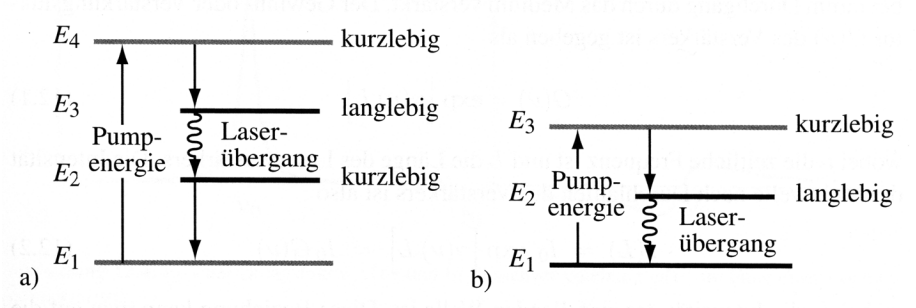
\includegraphics[width=0.7\textwidth]{content/images/Niveausysteme.png}
                \caption{Ein Vier-Niveau-System (a) und ein Drei-Niveau-System (b) im Vergleich~\cite{laserprinzipien}.}
                \label{fig:Niveausysteme}
            \end{figure}
            \FloatBarrier\noindent
            %%Beim \textbf{Drei-Niveau-System} pumpt ein externer physikalischer Prozess das System vom Grundzustand $\Psi_0$ in einen Zustand $\Psi_2$, sodass die Energiedifferenz $\symup{\Delta}E_{21}$ größer ist als die Energiedifferenz, auf der die spontant Emission betrieben werden soll.
            %Aus dem obersten Zustand $\Psi_2$ kann dasDaher System nun entweder mit der gewünschten Laserfrequenz in Zustand $\Psi_1$ zerfallen und danach in den Grundzustand relaxieren, oder zuerst in den Zustand $\Psi_1$ relaxieren und danach in den Grundzustand zerfallen durch Aussendung eines Photons auf der Laserfrequenz \cite[326]{haken_wolf_2004}.
            %In beiden Fällen muss der relaxierende Übergang eine sehr geringe mittlere Lebensdauer besitzen, der zum Lasen verwendete Übergang dafür eine relativ hohe mittlere Lebensdauer.
            %\\
            %Das Drei-Niveau-System besitzt den Nachteil, dass der Laser immer aus dem Grundzustand gepumpt werden muss. Da der Grundzustand stabil ist, ist viel Energie nötig, um die Besetzungsinversion herzustellen und aufrechtzuerhalten.
            \\
            Für diesen Versuch ist insbesondere das Vier-Niveau-System relevant.
            %Beim \textbf{Vier-Niveau-System} 
            %Dabei befindet sich der Niveauübergang, der zum Lasen verwendet wird, zwischen dem Grundzustand und dem höchsten der vier Zustände. 
            Dessen Funktionsprinzip wird durch \autoref{fig:Niveausysteme} deutlich:
            Das System wird extern ins Energieniveau $E_3$ gepumpt, von wo aus es mit kurzer Lebensdauer in das Niveau $E_2$ relaxiert.
            Der Übergang $E_{2\rightarrow 1}$ ist langlebig und wird zum Lasen verwendet. 
            %Nach der stimulierten Emission befindet sich das System anders als im Drei-Niveau-System noch nicht im Grundzustand. 
            Der letzte Übergang $E_{1\rightarrow 0}$ findet ebenfalls relaxierend statt und hat eine sehr kurze Lebensdauer.
            %Daher wird für dieses System weniger Energie benötigt, um die Besetzungsinversion aufrechtzuerhalten~\cite[44-45]{eichler_2015}.
            \\
        \subsubsection{Resonatoren}
        \label{sec:resonator}
            Um den Laserbetrieb aufrechtzuerhalten, müssen die Photonen, die die stimulierte Emission in axialer Richtung auslösen können, möglichst lange im aktiven Medium verweilen. 
            Dort stabilisiert sich der Laser, sodass die Besetzungsinversion und die stimulierte Emission im Gleichgewicht liegen. 
            %Spontane Emission sollte nicht mehr stattfinden, weshalb die Zeit zwischen Anregung und Emission möglichst kurz sein sollte.
            Um die kohärenten Photonen möglichst lange im Medium zu halten, werden an beiden Enden des Mediums Spiegel angebracht. 
            Eine solche Anordnung von Spiegeln heißt \textbf{Resonator}. 
            Die elektromagnetische Strahlung bildet im Resonator stehende Wellen, die der Bedingung
            \begin{equation}
                L = \frac{n\lambda}{2}\,\mathrm{,}\,\,\,n \in \mathbb{N}
                \label{eqn:resontor}
            \end{equation}
            genügen. 
            Dabei ist $L$ die Resonatorlänge, $\lambda$ die Wellenlänge des Laserlichts und $n$ die Wellenzahl, also die Anzahl der Maxima der stehenden Welle.
            Die Länge des Resonators muss deshalb auf die Wellenlänge des Lasers abgestimmt werden. 
            %Damit die Laserstrahlung im Resonator stehende Wellen bilden kann, ist also die Resonatorlänge entscheidend.
            %Da die Wellenlänge des Laserlichts in der Regel im dreistelligen Nanometer-Bereich liegt, haben schon kleine Änderungen der Resonatorlänge einen großen Einfluss auf die Stabilität des Lasers.
            %Allerdings bedeutet die kurze Wellenlänge ebenso, dass sich bei Resonatorlängen im Mikrometer-Bereich viele longitudinale Moden im Resonator ausbilden können.
            Um das Auskoppeln des Laserlichts aus dem Resonator zu ermöglichen, hat einer der beiden Spiegel einen leicht abgesenkten Reflektionsgrad.
            \\
            Dabei ist allerdings entscheidend, dass die Pumpleistung des Lasers größer ist, als die Verluste durch das Auskoppeln aus dem Resonator~\cite[402-405]{haken_wolf_2004}. %\textbf{PASST DAS SO MIT QUELLE?} Jetzt Ja
            %Durch diesen Spiegel wird ein Teil des Laserlichts aus dem Resonator gelassen und dem weiteren Strahlengang des Lasers zugeführt.
            %Wie viel Laserlicht transmittiert wird, hängt davon ab, wie viel Licht innerhalb des Resonators nötig ist, um die stimulierte Emission stabil zu halten und Energieverluste auszugleichen.
            %Bei niederenergetischen Lasern liegt der Transmissionskoeffizient typerscherweise bei $T = \qty{1}{\percent}$ oder weniger. 
            %Hochenergetische Laser können auch Transmissionskoeffizienten im zweistelligen Prozentbereich aufweisen \cite[255]{svelto_1998}.
    \subsection{Bandstruktur und Halbleiter}
        Der Diodenlaser nutzt als aktives Medium die aktive Schicht eines Halbleiterchips.
        Halbleiter sind diejenigen Materialien, bei denen die Fermi-Energie innerhalb der Bandlücke liegt~\cite[347 f.]{gross_marx_2022}. 
        Bei Halbleitern ist die Bandlücke meistens kleiner als $\qty{2}{\electronvolt}$, sodass sie schon ab Raumtemperatur Strom leiten können \cite[714]{ashcroft_2005}.
        %Die Bandstruktur ist eines der wichtigsten Konzepte der Festkörperphysik. Sie ergibt sich aus der Dispersionsrelation der Elektronen, die sich im Gitter eines Festkörpers bewegen, und ist somit
        %direkt von der Gitterstruktur abhängig. Dabei ist ebenfalls die Fermi-Energie von großer Bedeutung. Sie ist genau die Energie, bis zu der die möglichen Zustände bei Temperatur $T=\qty{0}{\kelvin}$
        %durch die Elektronen besetzt sind. Das letzte noch vollständig mit Elektronen befüllte Energieband heißt Valenzband, das nächsthöhere heißt Leitungsband. Die Elektronen in diesem Band tragen
        %zur elektrischen und thermischen Leitung bei. Liegt die Fermienergie nun innerhalb des Leitungsbandes, leitet das entsprechende Material sehr gut und ist somit ein Metall.
        %Liegt die Fermi-Energie bei einem Material zwischen dem Leitungs- und dem Valenzband - also in der sogenannten Bandlücke - dann handelt es sich dabei um einen Isolator oder einen Halbleiter,
        %da die Elektronen erst die Bandlücke überwinden müssen, um zur Leitung beitragen zu können.
        %Wenn die Bandlücke klein genug ist, dass einige Elektronen schon bei Raumtemperatur diese Bandlücke überwinden können, spricht man von einem Halbleiter \cite[147 f.]{gross_marx_2022}.
    \subsubsection{Dotierung eines Halbleiters}
        Ein Halbleiter ist dotiert, wenn er gezielt mit Fremdatomen verunreinigt ist. 
        %Dotierung ist bei vielen Anwendungen von Halbleitern nötig, da die Ladungsträgerdichten des reinen Halbleitermaterials oft
        %zu gering sind. 
        Bei dem Material der Verunreinigung wird zwischen Donatoren und Akzeptoren unterschieden. 
        Für Halbleiter der IV. Hauptgruppe werden als Donatoren Elemente der V. Hauptgruppe verwendet, da sie ein überschüssiges Valenzelektron besitzen, das nicht zur Bindung benötigt wird. 
        Dieses befindet sich zusätzlich im Leitungsband. Als Akzeptoren werden Elemente der III. Hauptgruppe verwendet, da sie für die Bindung ein Elektron zu wenig besitzen und dem Valenzband ein Loch hinzufügen. 
        Löcher sind dabei nicht besetzte Zustände bzw. fehlende Elektronen. 
        Die Energie des Grundzustandes des Donatoratoms liegt etwas unterhalb des Leitungsbandes und die des Akzeptoratoms etwas überhalb des Valenzbandes. 
        Somit ist eine Ionisierungsenergie nötig, um den jeweiligen Zustand ins Leitungs- bzw. Valenzband anzuregen.
        Ist ein dotierter Halbleiter hauptsächlich mit Donatoren dotiert, so wird er n-dotiert genannt. 
        Ist er hauptsächlich mit Akzeptoren dotiert, wird er p-dotiert gennant~\cite[503-506]{gross_marx_2022}.
    \subsubsection{p-n-Übergang}
    \label{sec:pnubergang}
    Grenzen eine p-dotierte und eine n-dotierte Schicht direkt aneinander, wird von einem p-n-Übergang gesprochen. Im thermischen Gleichgewicht müssen hier die Energiebänder verbogen sein, da 
    das chemische Potential im gesamten Material konstant sein muss. Die Bandlücke wird durch die Verschiebung der Bänder an der Grenze also kleiner~\cite[517]{gross_marx_2022}. 
    Eine schematische Darstellung dessen ist für getrennte p- und n-dotierte Halbleiter ist in \autoref{fig:pnvor} und für angrenzende p- und n-dotierte Hablleiterschichten 
    in \autoref{fig:pnnach} dargestellt. Auch die Energieniveaus der Grundzustände der jeweiligen Dotierung sind in der Grafik eingezeichnet. 
    \begin{figure} 
        \centering
        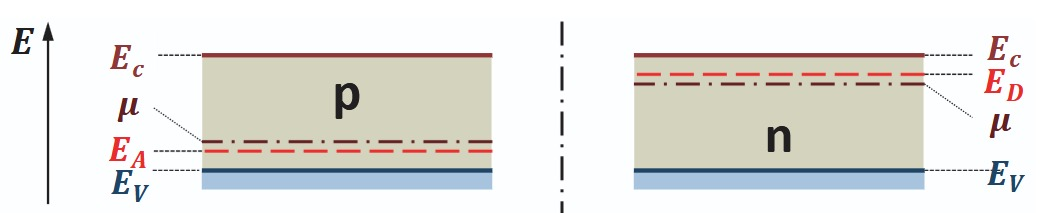
\includegraphics[width=0.7\textwidth]{content/images/pnvor.jpeg}
        \caption{Darstellung der Energiebänder sowei des chemischen Potenzials in getrennten p- und n-dotierten Halbleitern~\cite[519]{gross_marx_2022}.}% \cite{V60}
        \label{fig:pnvor}
    \end{figure}
    \begin{figure}
        \centering
        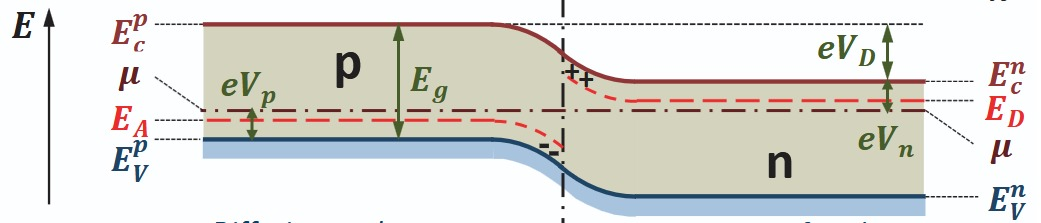
\includegraphics[width=0.7\textwidth]{content/images/pnnach.jpeg}
        \caption{Darstellung der Energiebänder sowei des chemischen Potenzials an der Grenze zwischen p- und n-dotierten Halbleiterschichten~\cite[519]{gross_marx_2022}.}% \cite{V60}
        \label{fig:pnnach}
    \end{figure}
    \\
    %Die Energiebänder bilden mit den Energieniveaus der Donatoren und Akzeptoren effektiv ein wie in Unterabschnitt \ref{sec:systeme} beschriebenes Vier-Zustands-System. 
    %Dabei ist der Grundzustand ein voll besetztes Energieband in der p-dotierten Schicht
    Dabei diffundieren einige der Elektronen der n-dotierten Schicht und einige der Löcher der p-dotierten Schicht an der Grenzfläche 
    in die jeweils andere Schicht. Dadurch entsteht der sog. Diffusionsstrom. Dieser wird im thermischen Gleichgewicht durch den Driftstrom kompensiert, welcher sich dadurch ergibt, 
    dass nahe der Grenze in der p-dotierten Schicht eine negative und in er n-dotierten Schicht eine positive Raumladungsdichte entsteht. Dieser Bereich wird Raumladungszone genannt~\cite[517-520]{gross_marx_2022}.
    \\
    %Liegt an dem Halbleiter eine Spannung an, fungiert er als Diode. 
    Liegt am p-n-Übergang eine Spannung so an, dass an der n-dotierten Schicht der Pluspol anliegt, wird die Raumladungszone an der Grenze
    größer, wodurch die Spannung an der Grenze abfällt, da bei steigender Spannung der Stromfluss abnimmt. Dies ist die Sperrrichtung der Diode. 
    Liegt der Minuspol an der n-dotierten Schicht an, wird die Raumladungszone kleiner. In dieser
    Richtung wird der fließende Strom mit steigender Spannung größer, weshalb dies die Durchlassrichtung ist~\cite[524-526]{gross_marx_2022}.
    \\
    Eine solche Halbleiterdiode kann nach dem Prinzip eines wie in Unterabschnitt~\ref{sec:systeme} beschriebenen Vier-Niveau-Systems Photonen emittieren. 
    Das Valenzband in der p-dotierten Schicht entspricht dem Grundzustand beim 
    Vier-Niveau-System. 
    Liegt an der Diode eine Spannung in Durchlassrichtung an, verschieben sich die Fermienergien der beiden Schichten. Es gelangen Elektronen ins Leitungsband der 
    p-Dotierten Schicht und Löcher ins Valenzband der n-dotierten Schicht. Das Leitungsband in der n-dotierten Schicht entspricht dem höchsten Energieniveau des
    Vier-Nivau-Systems. 
    Es entsteht durch die anliegende Spannung die für Laseraktivität benötigte Besetzungsinversion zwischen Grundzustand und höchstem Zustand. 
    Dies wird in \autoref{fig:pnjunciton} verdeutlicht. 
    Die Löcher und Elektronen relaxieren in Richtung der Grenze, wo sie anschließend miteinander rekombinieren und Photonen mit einer Energie aussenden, 
    die etwa der Bandlücke entspricht.
    Dies ist analog zu der Emission der beiden mittleren Energieniveaus im Vier-Nivau-System. 
    Der Bereich an der Grenzfläche, in welchem diese Emission stattfindet, wird aktiver Bereich genannt~\cite[396 f.]{svelto_1998}.
    \begin{figure}
        \centering
        \begin{subfigure}{0.3\textwidth}
          \centering
          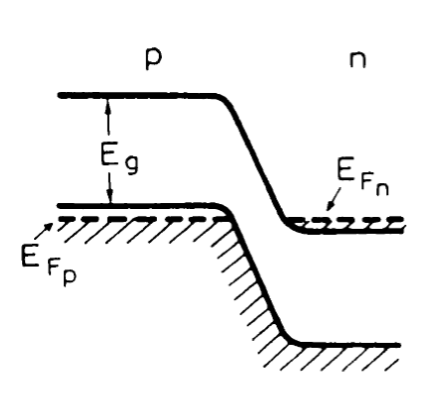
\includegraphics[width=\linewidth]{content/images/pnjunction1.png}
          \caption{Ohne anliegende Spannung.}
        \end{subfigure}
        \hfill
        \begin{subfigure}{0.3\textwidth}
          \centering
          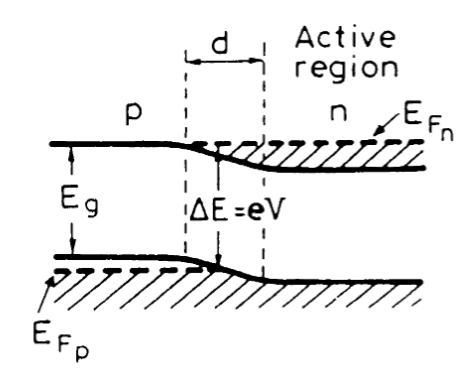
\includegraphics[width=\linewidth]{content/images/pnjunction2.png}
          \caption{Bei in Durchlassrichtung anliegender Spannung.}
        \end{subfigure}
        \caption{Schematische Darstellung der Energiebänder an der Grenzfläche mit und ohne in Durchlassrichtung anliegende Spannung~\cite[396]{svelto_1998}.}
        \label{fig:pnjunciton}
      \end{figure}
    \subsection{Der Diodenlaser}
    Um den Diodenlaser zu verstehen sind die folgenden vier Komponenten entscheidend:
    \subsubsection{Der Halbleiterchip}
    \label{sec:halbleiterchip}
    Das Herzstück des verwendeten Diodenlasers ist ein Halbleiterchip mit p- und n-dotierter Schicht. Hier findet genau der in Unterabschnitt~\ref{sec:pnubergang} beschriebene Prozess statt, wenn
    eine Spannung anliegt. Findet nur spontane Emission statt, ist die Diode in der LED-Phase (Light emitting diode). Die Wellenlänge der emittierten Photonen hängt von der Breite der 
    Bandlücke ab. Diese wiederum hängt sowohl vom Material des Halbleiters als auch, wie es aus Unterabschnitt~\ref{sec:pnubergang} hervorgeht, von der anliegenden Spannung ab. Auch die Temperatur 
    hat einen Einfluss auf die Energiebänder. 
    Das Material, dessen Temperatur und die anliegende Spannung geben einen groben Wellenlängenbereich vor, in dem sich das emittierte Licht der Diode befinden kann~\cite{V60}. 
    \subsubsection{Der Innere Resonator}
    Damit es zu Laseraktivität kommen kann bzw. die Diode in ihre Laserphase übergehen kann, muss die Emission, wie in Unterabschnitt~\ref{sec:resonator} erläutert, in einem Resonator 
    stattfinden. Nur so kann es zu stimulierter Emission und Lasing kommen. Innerhalb des Halbleiterchips gibt es einen Streifen, der als optischer Resonator dient.
    Dieser wird transversal durch Spaltflächen an den Rändern des Halbleiterchips begrenzt. Somit ist die Länge des Resonators und die Frequenzen, die durch ihn
    verstärkt werden, direkt von der Temperatur abhängig. In der Vertikalen wird das Licht dadurch innerhalb des Streifens gehalten, dass der Brechungsindex der aktiven Schicht höher ist als der 
    der umliegenden Schichten. In der Transversalen befinden sich ebenfalls Barrieren mit geringerem Brechungsindex. Die Periodizität der Verstärkung berechnet sich nach $\increment v_{\mathrm{FSR}}=\frac{c}{2Ln}$
    mit der Lichtgeschwindigkeit $c$, der Länge des Resonators $L$ und dem Brechungsindex $n$. Es ergibt sich ein Wert von $\increment v_{\mathrm{FSR}}\approx \qty{60}{\giga\hertz}$~\cite{V60}. 
    \label{sec:internalcavity}
    \subsubsection{Die Gitter-Rückkopplung}
    \label{sec:gratingfeedback}
    Das von der Diode ausgesendete Licht hat eine ellipsenförmige Wellenfront, welche sich ausbreitet, da sich das Licht an der Öffnung des internen Resonators mit rechteckigem Querschnitt beugt.
    %der interne Resonator einen rechteckigen Querschnitt hat.
    Das Laserlicht in der Diode ist kohärent und breitet sich nahezu axial aus. 
    %Daher kann für den Laserstrahl die Frauenhofer-Näherung angewandt werden. 
    %Die Form des Strahls nach der Beugung an der Rechteckblende ist beschrieben durch die Fouriertransformierte der Rechteckblendenfunktion. Diese ist ein Sinus Cardinalis in beiden transversalen Raumrichtungen.
    %Bei unterschiedlich langen Seiten des Rechtecks ergibt sich daher ein elliptischer Transversalschnitt des Laserstrahls nach der Beugung \cite[345]{demtröder_2026}.
    \\
    Um den elliptischen Strahl zu fokussieren, ist direkt hinter der Diode - wie in \autoref{fig:externallaser} zu erkennen - eine optische Linse 
    verbaut. Außerdem hat das Licht mit $\increment v \approx \qty{50}{\mega\hertz}$ noch eine zu große Bandbreite, weshalb ebenfalls ein Beugungsgitter verbaut ist. Dies ist 
    ebenfalls in \autoref{fig:externallaser} dargestellt. 
    Das Gitter reflektiert die nullte Beugungsordnung und damit ca. $15\%$ des Strahls zurück in den Diodenchip. Dadurch wird abhängig vom Gitterwinkel 
    ein Wellenlängenbereich mit deutlich kleinerer Bandbreite verstärkt und der Laser auf diese Wellenlänge stabilisiert. Die Beziehung zwischen Gitterwinkel und 
    Wellenlänge ist durch $\lambda = 2 d \mathrm{\sin}\theta$ gegeben. Die restlichen $85\%$ des Strahls werden, wie es durch \autoref{fig:externallaser} deutlich wird, nach
    außen Reflektiert und bilden den letztentlichen Laserstrahl~\cite{V60}. 
    \begin{figure}
        \centering
        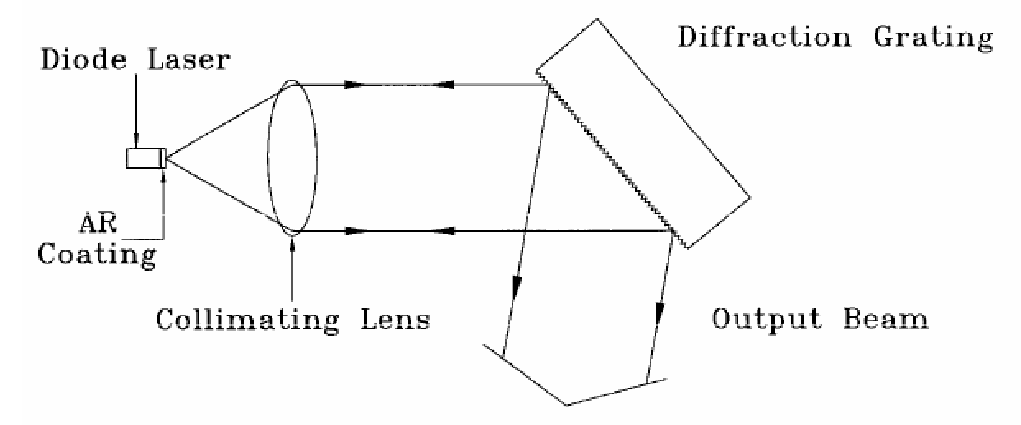
\includegraphics[width=0.7\textwidth]{content/images/grating.png}
        \caption{Dartstellung des Diodenlasers mit Beugungsgitter~\cite{V60}.}% \cite{V60}
        \label{fig:externallaser}
    \end{figure}
    \subsubsection{Der Äußerer Resonator}
    \label{sec:externalcavity}
    Das Beugungsgitter bildet mit dem gegenüberliegenden Ende des Diodenchips ebenfalls einen optischen Resonator. Dieser hat eine Länge von $\qty{15}{\milli\meter}$ und verstärkt
    Frequenzen mit einer Periodizität von $\increment v_{\mathrm{FSR}}\approx \qty{10}{\giga\hertz}$. Diese ist kleiner als die des inneren Resonators. 
    \\
    Da die Resonatorlänge hier um einen Faktor $10^5$ größer ist als die Wellenlänge des Laserlichts, bilden sich im externen Resonator sehr viele verschiedene longitudinale Moden aus - deutlich mehr als im internen Resonator. 
    
    \subsubsection{Nettoverstärkung}
    Die letztendliche Nettoverstärkung ergibt sich aus allen diesen Elementen. Dies ist in \autoref{fig:netgain} schematisch dargestellt. Dabei ist die mit \enquote{Medium} betitelte Verstärkung die in
    Unterabschnitt~\ref{sec:halbleiterchip} beschriebene allgemeine Verstärkung des Materials. Der interne Resonator aus  Unterabschnitt~\ref{sec:internalcavity} wird durch \enquote{Internal Cavity} dargestellt 
    und der äußere Resonator aus  Unterabschnitt~\ref{sec:externalcavity} durch \enquote{External Cavity}. Die schmale Verstärkung der Gitter-Rückkopplung aus  Unterabschnitt~\ref{sec:gratingfeedback} ist durch
    \enquote{Grating Feedback} repräsentiert.
    \begin{figure}
        \centering
        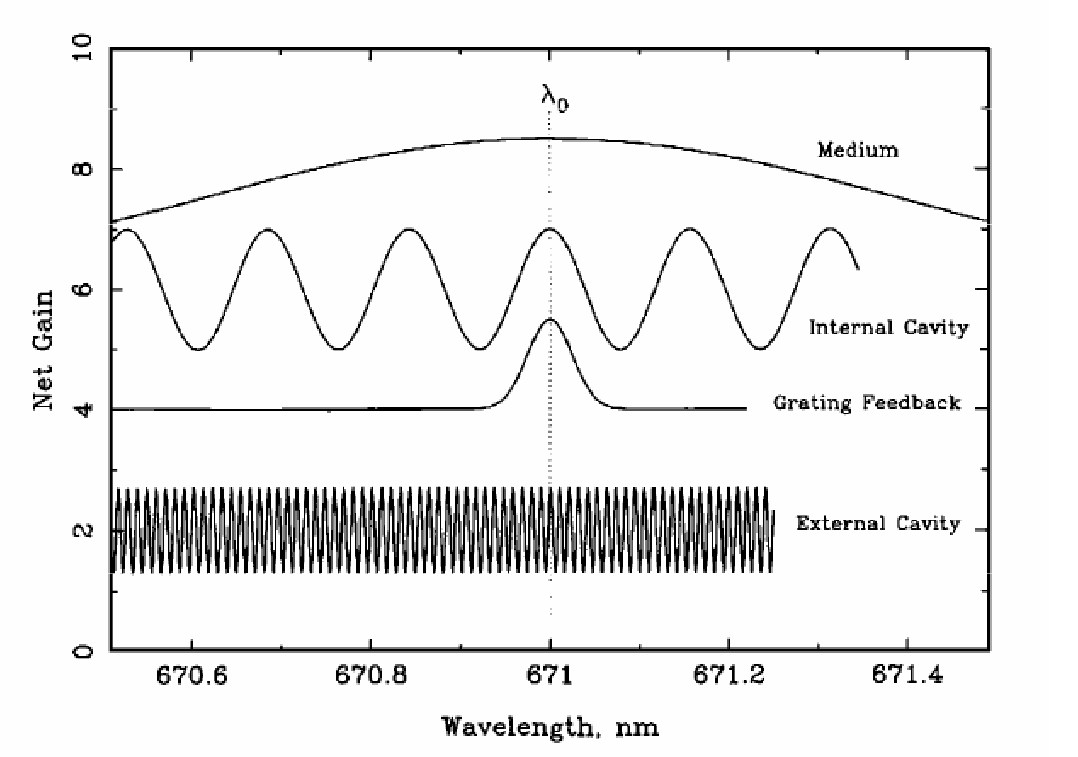
\includegraphics[width=0.7\textwidth]{content/images/netgain.png}
        \caption{Schematische Darstellung, wie die einzenlen Bauteile des Diodenlasers zur Vertärkung (net gain) bei verschiedenen Wellenlängen (wavelength) beitragen~\cite{V60}.}% 
        \label{fig:netgain}
    \end{figure}
    Es ist zu beachten, dass die tatsächliche Frequenz zwischen den einzelnen Moden der Resonatoren springen kann, da diese diskret sind. Dabei ist die Überlagerung der beiden
    Resonatoren und der Gitter-Rückkopplung, wie sie in \autoref{fig:modehop} dargestellt ist von Bedeutung. Verscheibt sich die Gitter-Rückkopplung durch Verstellen des Gitterwinkels 
    sodass die Verstärkung in der nächsten inneren Mode größer ist, springt der Laser in die nächste Mode.
    \begin{figure}
        \centering
        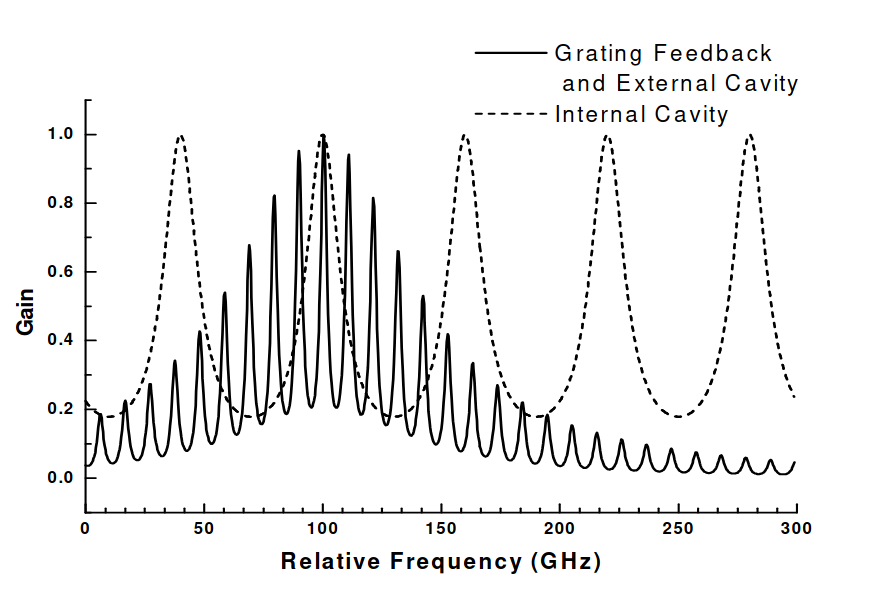
\includegraphics[width=0.7\textwidth]{content/images/modehop.png}
        \caption{Schematische Darstellung der Überlagerung der Nettoverstärkung mit verschiedenen Moden der beiden Resonatoren~\cite{V60}.}% \cite{V60}
        \label{fig:modehop}
    \end{figure}
    
    
